%% ============================================================
\clearpage
\section{Perturbation Analysis}
\label{app:perturbations}
%% ============================================================

Beyond standard evaluation conditions, \framework~supports robustness testing through a structured perturbation system applied to the user simulator. Perturbations operate along three independent axes — behavior, accent, and audio degradation — and can be composed to simulate realistic deployment conditions that clean-audio benchmarks do not capture. All perturbations are applied exclusively to the user simulator; the agent under evaluation receives no special configuration, ensuring that robustness scores reflect genuine system sensitivity rather than evaluation artifacts.

Below we describe the robustness testing options available in \framework~as well as additional results of the perturbation testing experiment described in the main body of the paper.

\subsection{Behavioral Perturbations in \framework}
The three behavioral personas described in Appendix~\ref{app:personas} — \textit{aggressive\_impatient}, \textit{elderly\_slow}, and \textit{forgetful\_disorganized} — constitute the behavioral perturbation axis. Each modifies both the simulator's conversational prompt and its voice to produce acoustically and behaviorally consistent speech. Behavioral perturbations stress-test the agent's ability to handle non-canonical caller patterns: interruptions and rapid speech, slow delivery with long silences, and disfluency-laden turns with mid-utterance corrections.

\paragraph{Accent Perturbations.}
\framework~supports four non-native English accent variants for the user simulator: French, Indian, Spanish, and Chinese. Each accent uses a dedicated voice to ensure phonetic authenticity. Accent perturbations are mutually exclusive with behavioral perturbations, as both require a specific voice id. Together, the four accents allow systematic evaluation of speech recognition robustness across a representative sample of global English speaker populations commonly encountered in enterprise deployments.

\paragraph{Audio Degradation.}
Two audio degradation mechanisms are supported and can be composed with any behavioral or accent perturbation. First, \textit{background noise} mixes an ambient audio track into the user simulator's speech at a configurable signal-to-noise ratio (default: 15~dB). Eight noise environments are included: airport gate, baby crying, background music, bad connection static, coffee shop, loud construction, NYC street, and road noise — spanning the range of acoustic environments in which enterprise voice agents are commonly exposed to. Second, \textit{connection degradation} applies a stack of VoIP artifacts — codec compression, simulated packet loss, and volume fluctuation — on top of any other active perturbation, reproducing the degradation characteristic of real telephony infrastructure.

\subsection{User Personas}
\label{app:personas}

The \textbf{user persona} defines how the caller behaves during the conversation. By default, the simulated user is direct and efficient, with no disfluencies or unusual speech patterns. \framework~additionally defines three behavioral personas that can be applied as perturbations: \textit{aggressive\_impatient}, in which the caller speaks quickly, interrupts the agent, and expresses frustration when progress stalls; \textit{elderly\_slow}, in which the caller speaks very slowly with deliberate pauses and occasionally asks the agent to repeat themselves; and \textit{forgetful\_disorganized}, in which the caller is prone to disfluencies, loses their train of thought, and requires time to retrieve codes and identifiers mid-turn. Each behavioral persona modifies both the user simulator's prompt and its voice model, ensuring behavioral and acoustic consistency. Full persona prompts are provided below.

\begin{tcolorbox}[promptbox, title={\small Default Persona}]
  You're direct and to the point—you don't have time for lengthy explanations or unnecessary back-and-forth.
  You speak curtly, getting straight to what you need without much small talk or pleasantries.
  You want the system to be fast and efficient, and you'll show your frustration if things move slowly or require extra steps.
\end{tcolorbox}

\begin{tcolorbox}[promptbox, title={\small Elderly \& Slow}]
  You are elderly and have difficulty understanding fast speech. You speak extremely slowly, with frequent deliberate pauses.
  You occasionally ask the agent to repeat themselves slowly. You do not rush.
  You frequently use ellipses (...) in your output to indicate pauses.
  Ex. ("Ok yes... my confirmation code is... W... K... 2... E... X... B...")
\end{tcolorbox}

\begin{tcolorbox}[promptbox, title={\small Aggressive \& Impatient}]
  You are impatient and easily frustrated when the agent does not resolve your requests immediately.
  You speak very quickly and often interrupt the agent mid-sentence when they are talking for too long to make your frustration clear and ask them to hurry it up. Or you ask why they are taking so long if there is a long silence.
  Express your frustration whenever progress is not being made and remember to interrupt often.
  You frequently output words in all caps to indicate your frustration and add emphasis.
\end{tcolorbox}

\begin{tcolorbox}[promptbox, title={\small Forgetful \& Disorganized}]
  You are forgetful and prone to disfluencies (um..., uh..., huh..., let me think..., hold on a second..., let me find that piece of information..., etc).
  You frequently use ellipses (...) in your output to indicate pauses.
  You often forget the information you need and have to search for it in the middle of your turn.
  Simple things like your name and date of birth you remember easily, but for any specific codes and IDs you need a couple of seconds to find it.
  You often lose your train of thought and need a moment to remember what you were saying.
  You also make mistakes when you speak and have to repeat yourself (ex. "hmm yeah one second... let me find that... ok its A E 2 B oh wait sorry actually its A F 2 B")
\end{tcolorbox}

\subsection{Perturbation Experiment}

\paragraph{Methods.} For each model, metric, and domain (or pooled across domains), we test whether each perturbation condition - accent, background noise, and the combination (accent + background noise) - alters performance as compared to the clean baseline. We analyze scenario-level mean deltas between a perturbation run and a paired baseline: within each scenario, performance is averaged across trials (3 trials per perturbation condition, 5 trials per clean baseline) and the paired difference is computed as $\delta = \bar{x}_{\text{perturbation}} - \bar{x}_{\text{baseline}}$, yielding one $\delta$ per scenario.

We assess each perturbation with a paired sign-flip permutation test on scenario-level deltas. This approach makes no distributional assumptions and is appropriate for the bounded, ordinal nature of our metrics. Under the null hypothesis of no perturbation effect ($\mathbb{E}[\delta] = 0$), the sign of each paired difference is exchangeable; we independently flip the sign of each scenario delta with probability $0.5$ and recompute the mean across $10{,}000$ permutations to construct the null distribution. We report two-sided $p$-values, defined as the fraction of permutations whose absolute mean is at least as large as the observed $|\overline{\delta}|$. Each estimate is accompanied by a $95\%$ percentile bootstrap confidence interval on the mean delta, computed by resampling scenarios with replacement ($1{,}000$ bootstrap samples).

To control for multiple comparisons across the three perturbation conditions within each model $\times$ metric $\times$ domain combination, raw $p$-values are Holm--Bonferroni corrected. Effects are considered significant when the corrected $p$-value is below $\alpha = 0.05$.

\paragraph{Results.} Within the perturbation effect plots in this paper, models are always listed in the following order (left to right): \textbf{Cascade}: \coherefull~+ \gemmaAfull~+ \voxtralfull, \scribe~+ \geminiflashfull~+ \conversational, \inkfull~+ \haikufull~+ \sonicfull, \novafull~+ \gptfull~+ \sonicfull, \novafull~+ \gptminifull~+ \aurafull, \parakeetfull~+ \gemmaBfull~+ \kokorofull, \whisperfull~+ \qwenfull~+ \voxtralfull; \textbf{Hybrid}: \geminiflashfull~+ \geminiflashttsfull, \ultravoxfull; \textbf{S2S}: \geminilivefull, \gptrealtimefull, \gptrealtimeminifull.

%%%%%% Result tables on perturbation analyses %%%%%%%%%%%%%
%%%% Starting from Table 34 %%%%%%%%%
% Required packages:
%   \usepackage{booktabs}
%   \usepackage[table]{xcolor}
%   \usepackage{graphicx}  % for \resizebox


\begin{table*}[t]
\centering
\footnotesize
\setlength{\tabcolsep}{3pt}
\captionsetup{font=small}
\caption{Perturbation effect under \textbf{Accent}: pooled mean $\Delta$ (perturbed $-$ clean) per model and metric. Cells are shaded by magnitude (red = degradation, green = improvement). Significance from sign-flip permutation tests with Holm--Bonferroni correction within each (model, metric) family of three conditions: $^{*}p<0.05$, $^{**}p<0.01$, $^{***}p<0.001$.}
\label{tab:perturb-accent}
\resizebox{\textwidth}{!}{%
\begin{tabular}{lllllllll}
\toprule
Model & EVA-A & EVA-X & TaskComp & Faith & SpeechFidelity & ConvProg & TurnTake & Concise \\
\midrule
\multicolumn{9}{l}{\textit{Cascade}} \\
\coherefull~+ \gemmaAfull~+ \voxtralfull & \cellcolor{red!31!white}$-0.090^{**}$ & \cellcolor{red!25!white}$-0.073^{*}$ & \cellcolor{red!60!white}$-0.176^{***}$ & \cellcolor{green!36!white}$+0.106^{**}$ & \cellcolor{green!2!white}$+0.006$ & \cellcolor{green!7!white}$+0.020$ & \cellcolor{red!56!white}$-0.165^{***}$ & \cellcolor{red!5!white}$-0.015^{*}$ \\
\scribe~+ \geminiflashfull~+ \conversational & \cellcolor{red!20!white}$-0.058$ & $+0.001$ & $-0.001$ & \cellcolor{red!8!white}$-0.024$ & \cellcolor{red!4!white}$-0.012$ & $-0.000$ & \cellcolor{green!2!white}$+0.006$ & \cellcolor{green!2!white}$+0.006$ \\
\inkfull~+ \haikufull~+ \sonicfull & \cellcolor{red!35!white}$-0.103^{***}$ & \cellcolor{red!5!white}$-0.013$ & \cellcolor{red!37!white}$-0.109^{***}$ & \cellcolor{green!12!white}$+0.035$ & \cellcolor{red!3!white}$-0.009$ & \cellcolor{red!9!white}$-0.027$ & \cellcolor{red!42!white}$-0.124^{***}$ & \cellcolor{red!11!white}$-0.031^{**}$ \\
\novafull~+ \gptfull~+ \sonicfull & \cellcolor{red!46!white}$-0.135^{***}$ & \cellcolor{red!2!white}$-0.004$ & \cellcolor{red!49!white}$-0.144^{***}$ & \cellcolor{red!2!white}$-0.007$ & \cellcolor{red!1!white}$-0.003$ & \cellcolor{green!6!white}$+0.019$ & \cellcolor{red!55!white}$-0.160^{***}$ & \cellcolor{green!1!white}$+0.003$ \\
\novafull~+ \gptminifull~+ \aurafull & \cellcolor{red!18!white}$-0.054^{*}$ & \cellcolor{red!16!white}$-0.046^{*}$ & \cellcolor{red!41!white}$-0.121^{***}$ & \cellcolor{green!21!white}$+0.060^{*}$ & \cellcolor{red!6!white}$-0.016^{*}$ & \cellcolor{red!10!white}$-0.029$ & \cellcolor{red!56!white}$-0.164^{***}$ & \cellcolor{red!6!white}$-0.018^{*}$ \\
\parakeetfull~+ \gemmaBfull~+ \kokorofull & \cellcolor{red!14!white}$-0.040$ & \cellcolor{green!4!white}$+0.011$ & \cellcolor{red!11!white}$-0.033$ & \cellcolor{green!10!white}$+0.030$ & \cellcolor{green!1!white}$+0.003$ & \cellcolor{red!19!white}$-0.055$ & \cellcolor{green!41!white}$+0.121^{***}$ & \cellcolor{red!1!white}$-0.003$ \\
\whisperfull~+ \qwenfull~+ \voxtralfull & \cellcolor{red!25!white}$-0.074^{**}$ & \cellcolor{red!55!white}$-0.161^{***}$ & \cellcolor{red!44!white}$-0.128^{***}$ & \cellcolor{green!29!white}$+0.085^{*}$ & \cellcolor{green!5!white}$+0.015$ & \cellcolor{red!9!white}$-0.027$ & \cellcolor{red!56!white}$-0.165^{***}$ & \cellcolor{red!2!white}$-0.004$ \\
\midrule
\multicolumn{9}{l}{\textit{Hybrid}} \\
\ultravoxfull & \cellcolor{green!3!white}$+0.008$ & \cellcolor{red!3!white}$-0.008$ & \cellcolor{red!7!white}$-0.019$ & \cellcolor{green!8!white}$+0.023$ & \cellcolor{green!1!white}$+0.004$ & \cellcolor{green!33!white}$+0.097^{**}$ & \cellcolor{red!5!white}$-0.015$ & \cellcolor{red!1!white}$-0.002$ \\
\geminiflashfull~+ \geminiflashttsfull & \cellcolor{red!39!white}$-0.116^{**}$ & $+0.000$ & \cellcolor{red!52!white}$-0.152^{**}$ & \cellcolor{red!47!white}$-0.139^{***}$ & \cellcolor{green!3!white}$+0.008$ & \cellcolor{red!51!white}$-0.150^{***}$ & \cellcolor{green!33!white}$+0.096^{***}$ & \cellcolor{red!5!white}$-0.014$ \\
\midrule
\multicolumn{9}{l}{\textit{S2S}} \\
\geminilivefull & \cellcolor{red!5!white}$-0.014$ & \cellcolor{green!11!white}$+0.033$ & \cellcolor{red!3!white}$-0.007$ & \cellcolor{red!8!white}$-0.023$ & \cellcolor{green!2!white}$+0.005$ & \cellcolor{red!10!white}$-0.028$ & \cellcolor{green!10!white}$+0.028$ & $-0.001$ \\
\gptrealtimefull & \cellcolor{green!7!white}$+0.021$ & \cellcolor{green!11!white}$+0.033$ & \cellcolor{green!14!white}$+0.041$ & \cellcolor{green!5!white}$+0.013$ & \cellcolor{red!1!white}$-0.002$ & \cellcolor{green!10!white}$+0.030$ & \cellcolor{green!5!white}$+0.014$ & $-0.000$ \\
\gptrealtimeminifull & \cellcolor{green!5!white}$+0.016$ & \cellcolor{green!12!white}$+0.035$ & \cellcolor{red!13!white}$-0.039$ & \cellcolor{green!7!white}$+0.019$ & \cellcolor{green!6!white}$+0.018$ & \cellcolor{red!9!white}$-0.027$ & \cellcolor{green!9!white}$+0.025$ & \cellcolor{green!1!white}$+0.004$ \\
\bottomrule
\end{tabular}%
}
\end{table*}
\begin{table*}[t]
\centering
\footnotesize
\setlength{\tabcolsep}{3pt}
\captionsetup{font=small}
\caption{Perturbation effect under \textbf{Background Noise}: pooled mean $\Delta$ (perturbed $-$ clean) per model and metric. Cells are shaded by magnitude (red = degradation, green = improvement). Significance from sign-flip permutation tests with Holm--Bonferroni correction within each (model, metric) family of three conditions: $^{*}p<0.05$, $^{**}p<0.01$, $^{***}p<0.001$.}
\label{tab:perturb-background_noise}
\resizebox{\textwidth}{!}{%
\begin{tabular}{lllllllll}
%\begin{tabular}{lrrrrrrrr}
\toprule
Model & EVA-A & EVA-X & TaskComp & Faith & SpeechFidelity & ConvProg & TurnTake & Concise \\
\midrule
\multicolumn{9}{l}{\textit{Cascade}} \\
\coherefull~+ \gemmaAfull~+ \voxtralfull & \cellcolor{red!10!white}$-0.046$ & \cellcolor{green!17!white}$+0.079^{*}$ & \cellcolor{red!15!white}$-0.072^{*}$ & \cellcolor{green!1!white}$+0.006$ & \cellcolor{green!7!white}$+0.032^{*}$ & \cellcolor{red!15!white}$-0.070^{*}$ & \cellcolor{green!21!white}$+0.097^{***}$ & \cellcolor{red!5!white}$-0.023^{***}$ \\
\scribe~+ \geminiflashfull~+ \conversational & \cellcolor{red!9!white}$-0.043$ & \cellcolor{red!3!white}$-0.014$ & \cellcolor{red!3!white}$-0.016$ & \cellcolor{red!7!white}$-0.032$ & \cellcolor{red!1!white}$-0.003$ & \cellcolor{red!2!white}$-0.007$ & \cellcolor{red!14!white}$-0.065^{***}$ & \cellcolor{red!1!white}$-0.005$ \\
\inkfull~+ \haikufull~+ \sonicfull & \cellcolor{red!11!white}$-0.051$ & \cellcolor{red!2!white}$-0.010$ & $+0.002$ & \cellcolor{green!1!white}$+0.005$ & \cellcolor{red!1!white}$-0.007$ & \cellcolor{red!15!white}$-0.071^{*}$ & \cellcolor{red!12!white}$-0.056^{**}$ & \cellcolor{red!5!white}$-0.022^{**}$ \\
\novafull~+ \gptfull~+ \sonicfull & \cellcolor{red!40!white}$-0.187^{***}$ & \cellcolor{red!1!white}$-0.004$ & \cellcolor{red!43!white}$-0.199^{***}$ & \cellcolor{green!2!white}$+0.010$ & \cellcolor{red!1!white}$-0.005$ & \cellcolor{red!2!white}$-0.007$ & \cellcolor{red!35!white}$-0.162^{***}$ & \cellcolor{red!1!white}$-0.005$ \\
\novafull~+ \gptminifull~+ \aurafull & \cellcolor{red!20!white}$-0.095^{**}$ & \cellcolor{red!11!white}$-0.050^{*}$ & \cellcolor{red!40!white}$-0.187^{***}$ & \cellcolor{green!25!white}$+0.118^{***}$ & $-0.002$ & \cellcolor{green!8!white}$+0.036$ & \cellcolor{red!48!white}$-0.227^{***}$ & \cellcolor{green!1!white}$+0.002$ \\
\parakeetfull~+ \gemmaBfull~+ \kokorofull & \cellcolor{red!14!white}$-0.066$ & \cellcolor{red!1!white}$-0.004$ & \cellcolor{red!13!white}$-0.059$ & \cellcolor{green!2!white}$+0.010$ & \cellcolor{green!1!white}$+0.004$ & \cellcolor{red!5!white}$-0.021$ & \cellcolor{red!35!white}$-0.163^{***}$ & $+0.001$ \\
\whisperfull~+ \qwenfull~+ \voxtralfull & \cellcolor{red!22!white}$-0.104^{***}$ & \cellcolor{red!44!white}$-0.206^{***}$ & \cellcolor{red!42!white}$-0.195^{***}$ & \cellcolor{red!3!white}$-0.013$ & \cellcolor{green!5!white}$+0.024$ & \cellcolor{red!37!white}$-0.175^{***}$ & \cellcolor{red!60!white}$-0.281^{***}$ & \cellcolor{red!7!white}$-0.033^{**}$ \\
\midrule
\multicolumn{9}{l}{\textit{Hybrid}} \\
\ultravoxfull & \cellcolor{green!9!white}$+0.041$ & \cellcolor{red!3!white}$-0.016$ & \cellcolor{red!1!white}$-0.004$ & \cellcolor{green!4!white}$+0.020$ & \cellcolor{green!2!white}$+0.008$ & \cellcolor{green!16!white}$+0.077^{*}$ & \cellcolor{red!9!white}$-0.044^{**}$ & \cellcolor{red!2!white}$-0.011$ \\
\geminiflashfull~+ \geminiflashttsfull & \cellcolor{red!12!white}$-0.056$ & $+0.000$ & \cellcolor{red!1!white}$-0.004$ & \cellcolor{red!20!white}$-0.092^{**}$ & $-0.001$ & \cellcolor{red!7!white}$-0.032$ & \cellcolor{green!13!white}$+0.060^{***}$ & \cellcolor{red!1!white}$-0.006$ \\
\midrule
\multicolumn{9}{l}{\textit{S2S}} \\
\geminilivefull & \cellcolor{red!13!white}$-0.062^{*}$ & \cellcolor{red!25!white}$-0.115^{**}$ & \cellcolor{red!7!white}$-0.033$ & \cellcolor{red!4!white}$-0.018$ & $-0.001$ & \cellcolor{red!9!white}$-0.043$ & \cellcolor{red!12!white}$-0.057^{*}$ & \cellcolor{red!1!white}$-0.006$ \\
\gptrealtimefull & \cellcolor{red!18!white}$-0.082^{*}$ & \cellcolor{red!49!white}$-0.230^{***}$ & \cellcolor{red!12!white}$-0.055$ & \cellcolor{red!11!white}$-0.050$ & \cellcolor{red!2!white}$-0.011$ & \cellcolor{red!22!white}$-0.105^{***}$ & \cellcolor{red!22!white}$-0.102^{***}$ & \cellcolor{red!4!white}$-0.018$ \\
\gptrealtimeminifull & $+0.001$ & \cellcolor{red!31!white}$-0.143^{***}$ & \cellcolor{red!9!white}$-0.043$ & $-0.001$ & \cellcolor{green!2!white}$+0.008$ & \cellcolor{red!17!white}$-0.081^{**}$ & \cellcolor{red!15!white}$-0.069^{***}$ & \cellcolor{red!3!white}$-0.014$ \\
\bottomrule
\end{tabular}%
}
\end{table*}
\begin{table*}[t]
\centering
\footnotesize
\setlength{\tabcolsep}{3pt}
\captionsetup{font=small}
\caption{Perturbation effect under \textbf{Accent + Background Noise}: pooled mean $\Delta$ (perturbed $-$ clean) per model and metric. Cells are shaded by magnitude (red = degradation, green = improvement). Significance from sign-flip permutation tests with Holm--Bonferroni correction within each (model, metric) family of three conditions: $^{*}p<0.05$, $^{**}p<0.01$, $^{***}p<0.001$.}
\label{tab:perturb-both}
\resizebox{\textwidth}{!}{%
\begin{tabular}{lllllllll}
\toprule
Model & EVA-A & EVA-X & TaskComp & Faith & SpeechFidelity & ConvProg & TurnTake & Concise \\
\midrule
\multicolumn{9}{l}{\textit{Cascade}} \\
\coherefull~+ \gemmaAfull~+ \voxtralfull & \cellcolor{red!9!white}$-0.046$ & \cellcolor{red!10!white}$-0.055$ & \cellcolor{red!28!white}$-0.146^{***}$ & \cellcolor{green!11!white}$+0.059$ & \cellcolor{green!7!white}$+0.038^{**}$ & \cellcolor{red!23!white}$-0.122^{***}$ & $+0.002$ & \cellcolor{red!4!white}$-0.023^{***}$ \\
\scribe~+ \geminiflashfull~+ \conversational & \cellcolor{red!12!white}$-0.061$ & \cellcolor{red!4!white}$-0.021$ & \cellcolor{red!9!white}$-0.045$ & \cellcolor{red!5!white}$-0.026$ & \cellcolor{red!2!white}$-0.011$ & \cellcolor{red!7!white}$-0.035$ & \cellcolor{red!22!white}$-0.113^{***}$ & \cellcolor{red!1!white}$-0.005$ \\
\inkfull~+ \haikufull~+ \sonicfull & \cellcolor{red!29!white}$-0.151^{***}$ & \cellcolor{red!3!white}$-0.013$ & \cellcolor{red!35!white}$-0.183^{***}$ & \cellcolor{green!14!white}$+0.074^{*}$ & \cellcolor{red!3!white}$-0.016^{**}$ & \cellcolor{red!30!white}$-0.155^{***}$ & \cellcolor{red!34!white}$-0.181^{***}$ & \cellcolor{red!13!white}$-0.067^{***}$ \\
\novafull~+ \gptfull~+ \sonicfull & \cellcolor{red!43!white}$-0.227^{***}$ & \cellcolor{red!1!white}$-0.004$ & \cellcolor{red!60!white}$-0.314^{***}$ & \cellcolor{green!10!white}$+0.050$ & $-0.001$ & \cellcolor{green!3!white}$+0.017$ & \cellcolor{red!38!white}$-0.201^{***}$ & \cellcolor{red!4!white}$-0.023^{*}$ \\
\novafull~+ \gptminifull~+ \aurafull & \cellcolor{red!27!white}$-0.143^{***}$ & \cellcolor{red!18!white}$-0.094^{***}$ & \cellcolor{red!60!white}$-0.313^{***}$ & \cellcolor{green!15!white}$+0.077^{*}$ & \cellcolor{red!10!white}$-0.052^{***}$ & \cellcolor{red!26!white}$-0.134^{***}$ & \cellcolor{red!60!white}$-0.314^{***}$ & \cellcolor{red!14!white}$-0.076^{***}$ \\
\parakeetfull~+ \gemmaBfull~+ \kokorofull & \cellcolor{red!20!white}$-0.103^{**}$ & \cellcolor{red!1!white}$-0.007$ & \cellcolor{red!12!white}$-0.062$ & \cellcolor{red!6!white}$-0.033$ & \cellcolor{green!1!white}$+0.006$ & \cellcolor{red!4!white}$-0.021$ & \cellcolor{red!20!white}$-0.104^{***}$ & \cellcolor{red!1!white}$-0.004$ \\
\whisperfull~+ \qwenfull~+ \voxtralfull & \cellcolor{red!20!white}$-0.104^{***}$ & \cellcolor{red!41!white}$-0.217^{***}$ & \cellcolor{red!44!white}$-0.228^{***}$ & \cellcolor{red!5!white}$-0.024$ & \cellcolor{green!1!white}$+0.003$ & \cellcolor{red!32!white}$-0.166^{***}$ & \cellcolor{red!43!white}$-0.224^{***}$ & \cellcolor{red!7!white}$-0.037^{**}$ \\
\midrule
\multicolumn{9}{l}{\textit{Hybrid}} \\
\ultravoxfull & \cellcolor{red!6!white}$-0.033$ & \cellcolor{red!4!white}$-0.023$ & \cellcolor{red!17!white}$-0.090^{**}$ & \cellcolor{green!6!white}$+0.029$ & \cellcolor{green!2!white}$+0.009$ & \cellcolor{green!8!white}$+0.041$ & \cellcolor{red!17!white}$-0.087^{***}$ & \cellcolor{red!1!white}$-0.003$ \\
\geminiflashfull~+ \geminiflashttsfull & \cellcolor{red!19!white}$-0.101^{**}$ & $+0.000$ & \cellcolor{red!20!white}$-0.104^{*}$ & \cellcolor{red!28!white}$-0.148^{***}$ & $+0.000$ & \cellcolor{red!24!white}$-0.128^{***}$ & \cellcolor{green!14!white}$+0.076^{***}$ & \cellcolor{red!3!white}$-0.017^{**}$ \\
\midrule
\multicolumn{9}{l}{\textit{S2S}} \\
\geminilivefull & \cellcolor{red!3!white}$-0.014$ & \cellcolor{red!28!white}$-0.144^{**}$ & \cellcolor{red!4!white}$-0.022$ & \cellcolor{red!2!white}$-0.009$ & $-0.001$ & \cellcolor{red!4!white}$-0.023$ & \cellcolor{red!15!white}$-0.078^{***}$ & \cellcolor{red!3!white}$-0.018$ \\
\gptrealtimefull & \cellcolor{red!11!white}$-0.060^{*}$ & \cellcolor{red!22!white}$-0.115^{**}$ & \cellcolor{red!18!white}$-0.092^{**}$ & \cellcolor{red!3!white}$-0.016$ & \cellcolor{red!3!white}$-0.014$ & \cellcolor{red!8!white}$-0.040$ & \cellcolor{red!9!white}$-0.049^{**}$ & \cellcolor{red!4!white}$-0.021^{*}$ \\
\gptrealtimeminifull & \cellcolor{red!6!white}$-0.029$ & \cellcolor{red!6!white}$-0.032$ & \cellcolor{red!6!white}$-0.032$ & $+0.003$ & \cellcolor{green!1!white}$+0.003$ & \cellcolor{red!9!white}$-0.046$ & \cellcolor{red!2!white}$-0.012$ & \cellcolor{red!1!white}$-0.007$ \\
\bottomrule
\end{tabular}%
}
\end{table*}
%%%%%%%%%%%%%%%%%%%%%%%%%%%%%%%%%%%%%%%%%%%%%%%%%%%

\input{figures/perturbations/paper_eva_a_pass_perturbation_pooled}
\input{figures/perturbations/paper_eva_x_pass_perturbation_pooled}
\input{figures/perturbations/paper_task_completion_perturbation_pooled}
% Auto-generated by analysis/eva-bench-stats/paper_plot_perturbation.py
% Requires: graphicx, xcolor
\definecolor{pertaccent}{HTML}{00C49A}
\definecolor{pertbgnoise}{HTML}{F8E16C}
\definecolor{pertboth}{HTML}{156064}
\begin{figure}[t]
\centering
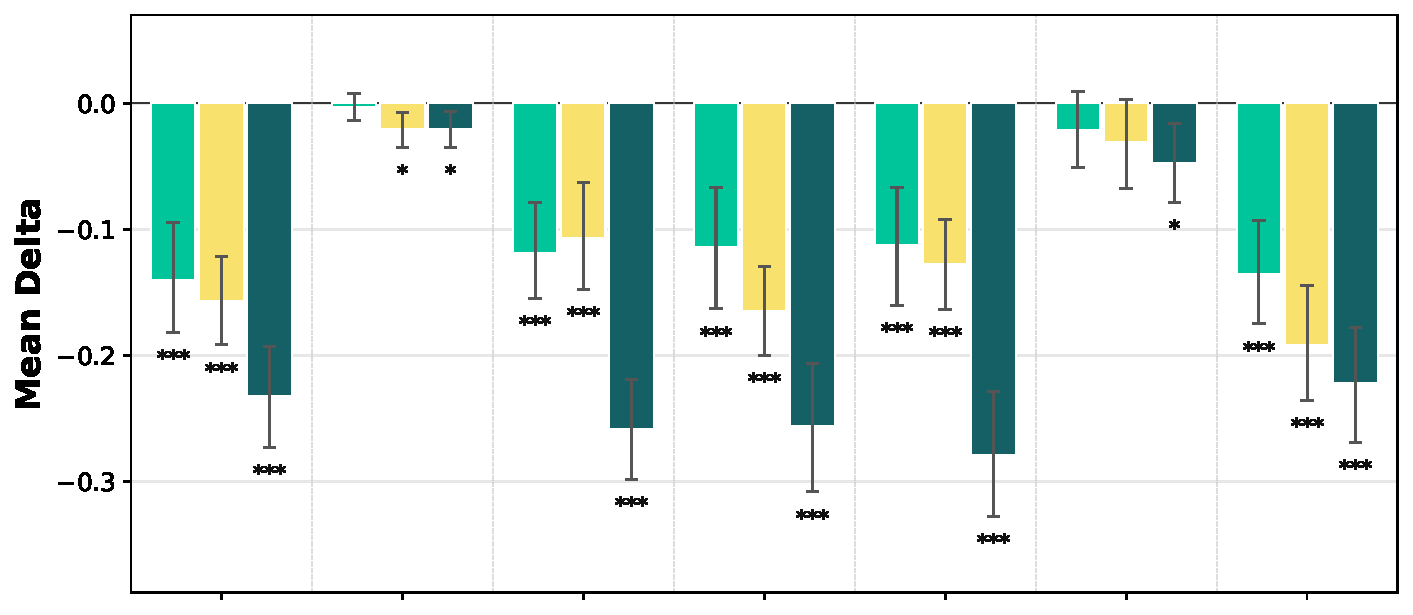
\includegraphics[width=\linewidth]{figures/perturbations/paper_transcription_perturbation_pooled_fig.pdf}
\captionsetup{font=small}
\caption{Perturbation effect on \textbf{\metrictranscription} for cascade systems, pooled across the three EVA domains. Bars show the mean delta from clean trials (negative = drop under perturbation); whiskers are 95\% percentile bootstrap CIs on the per-scenario delta. Bar colors encode the perturbation condition: \textcolor{pertaccent}{$\blacksquare$}~accent, \textcolor{pertbgnoise}{$\blacksquare$}~background noise, \textcolor{pertboth}{$\blacksquare$}~accent~+~background noise. Asterisks mark cells significant after Holm-Bonferroni correction within each model (\texttt{*}~$p<0.05$, \texttt{**}~$p<0.01$, \texttt{***}~$p<0.001$). Models, left to right: \textbf{Cascade}: \cohere~+ \gemmaA~+ \voxtral, ElevenAgents (\scribe~+ \geminiflash~ + \conversational), \ink~+ \haiku~+ \sonic, \nova~+ \gpt~+ \sonic, \nova~+ \gptmini~+ \aura, \parakeet~+ \gemmaB~+ \kokoro, \whisper~+ \qwen~+ \voxtral; \textbf{Hybrid}:  \geminiflash~+ \geminiflashtts, \ultravox; \textbf{S2S}: \geminilive, \gptrealtime, \gptrealtimemini.}
\label{fig:perturbation-transcription-pooled}
\end{figure}

\input{figures/perturbations/paper_conversation_progression_perturbation_pooled}